\chapter{\sffamily Distributed state networks}

{\bfseries\sffamily Concept.} The idea here is 

\textcolor{red}{This distributed state network archetype would make sense in simulations of brain, power, water or traffic networks.}

\section{\sffamily A large-scale Lotka-Volterra model}

\begin{figure}[h]
\centering
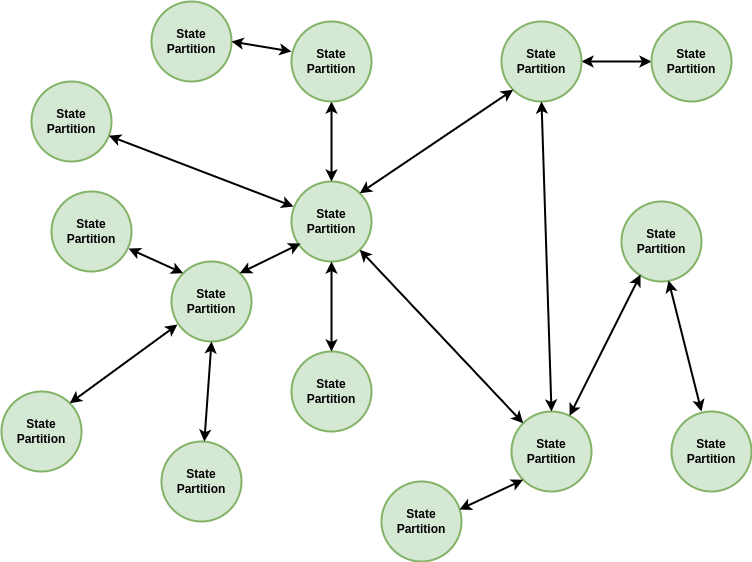
\includegraphics[width=12cm]{images/chapter-8-state-partition-graph.drawio.png}
\caption{State partition graph topology for distributed state network archetypes.}
\label{fig:state-partition-graph-distributed-state-networks}
\end{figure}

\textcolor{red}{
\begin{itemize}
\item{Full sim: full population-based spatial stochastic model}
\item{Inference model: mean field network inference features using the probabilistic reweighting using exponential weighting and cross-correlations}
\item{Also use the likelihood-free inference model and amortized full sim inference method.}
\end{itemize}
}

Inspired by the empirical dynamical modeling approach to sockeye salmon in Ref.~\cite{ye2015equation}, but also desiring a generative model which has some link to the classic causal models promoted by mathematical ecology; the goal here is to create and calibrate a stochastic model which predicts the fish counts, weights, lengths and ages for each species in each area based on the past system states. To do this, we will combine some well-known models from mathematical ecology with supervised learning.

The one-step master equation for the proposed stochastic simulation is given implictly by

\begin{align}
\frac{{\rm d}}{{\rm d} t} P(\dots, n_{i}, \dots, t) &= \sum_{\forall i}{\cal T}^{+}_{i}(\dots, n_i-1, \dots, {\sf f}, t)P(\dots, n_{i}-1, \dots, t) \\
&+ \sum_{\forall i}{\cal T}^{-}_{i}(\dots, n_i+1, \dots, {\sf f}, t)P(\dots, n_{i}+1, \dots, t) \\
&- \sum_{\forall i}\bigg[ {\cal T}^{+}_{i}(\dots, n_i, \dots, {\sf f}, t) + {\cal T}^{-}_{i}(\dots, n_i, \dots, {\sf f}, t) \bigg] P(\dots, n_{i}, \dots,t) \,,
\end{align}

where the time $t$ is defined in units of years and ${\cal T}^{+}_{i}$ and ${\cal T}^{-}_{i}$ are the transition coefficients for the $i$-th species, which depend not only on the counts for all species $n_1, n_2, \dots$, but also (in principle) on a larger feature space ${\sf f}$ generated by the available data up to time $t$.

The famous Lotka-Volterra system, with some modficiations for fishing and a larger set of species, would suggest transition coefficients of the form


\begin{align}
{\cal T}^{+}_{i}(\dots, n_i, \dots, {\sf f}, t) = {\cal T}^{+}_{i}(\dots, n_i, \dots) &= \Lambda_{i}(n_{i}) + n_{i}\alpha_{i}\sum_{\forall i' \, {\sf prey}}n_{i'}\\
{\cal T}^{-}_{i}(\dots, n_i, \dots, {\sf f}, t) = {\cal T}^{-}_{i}(\dots, n_i, \dots) &= n_{i}\mu_{i} +  n_{i}\gamma_{i} + n_{i}\beta_{i} \sum_{\forall i' \, {\sf pred}} n_{i'} \,,
\end{align}


where: $\Lambda_{i}(n_{i}) = \tilde{\Lambda_{i}}n_{i}e^{-\lambda_i(n_{i}-1)}$ is the density-dependent birth rate; $\mu_{i}$ is the species death rate; $\alpha_{i}$ is the increase in the baseline birth rate per fish caused by the increase in prey population; $\beta_{i}$ is the rate per fish of predation of the species; and $\gamma_{i}$ accounts for the rate of recreational fishing per fish of the species. To approach the present data-driven simulation problem, we're going to generalise this model by training ${\cal T}^{+}_{i}(\dots, n_i, \dots, {\sf f}, t)$ and ${\cal T}^{-}_{i}(\dots, n_i, \dots, {\sf f}, t)$ directly from the data and generated features.

Look into the likelihood from, e.g., an electrofishing survey such as in Ref.~\cite{envagency2015}...

\begin{align}
{\sf Likelihood} &= \sum_{{\sf data}}{\rm NB}\big[{\sf data};w_{i,{\sf survey}}\langle n_i(t_{{\sf data}})\rangle,k_{i,{\sf survey}}\big] \,,
\end{align}